%----------------------------------------------------------------------------------------
%	CHAPTER
%----------------------------------------------------------------------------------------

\chapterimage{chapter_head_2.pdf} % Chapter heading image

\chapter{More examples}
In this chapter we will present some data structure of AgvManager and some examples on agv scripting. In this chapter we will show only piece of code necessary to explain the concepts. Complete examples are provided with this document. The expamples package is divided by folders, every folder contain the script files. Mainly every example at least have 3 files: main.xs, common.xs and agvEventFunctions.xs. We will indicate in which file and function every piece of code can be found.

In AgvManager documentation we can find functions and data structures divided by argument, it means functions to manage vehicles, maps, databases, etc. Refer to the official documentation in order to get a complete list of functions and data structures.

An Agv usually transport a loading unit (UDC, LU) e.g. pallet, trolley, etc. , or a loading unit with a load on it e.g. a pallet with some mechanical parts on it.

For the presence Loading unit we find the variable bPresenza or bPres.
For the presense of a load on board of the Loading Unit (UDC) we find the variable bVasiPieni.

Data structures and constants definition can be found in \textcolor{red}{Script editor - All functions}.
%----------------------------------------------------------------------------------------
%	 Data structures
%----------------------------------------------------------------------------------------
\section{Xscript Agv Data structures}
In the documentation under the voice \textcolor{blue}{Estensione x-script per AgvManager » Funzioni per la gestione degli agv}, we can find some functions and data structures to manage AGVs. Here will present some data structures and functions that can operate on them.

Note that AgvManager have internal data structures where to save informations about vehicles, maps, points, etc. When we need, for example to get information about agv number 4, we create a strucutre similar to the one AgvManager have and by calling a dedicated function we can get information on Agv 4.

%------------------
%
%------------------
\subsection{XMapParams}
This structures contains some fields to define the dimensions of an AGV and movement behavior. There are two functions that operate on this structure to get information from AgvManger and set information to it.
For example, if we define a variable \textcolor{blue}{mPar} as: \textcolor{blue}{XMapParams mPar}, we can read parameter from AgvManager and store them into this structure by calling the function \textcolor{blue}{AgvGetMapParams(@mpar)}.
If we need to modify some parameter we can we use the dot operator of the structure.
To apply modification onto AgvManager we have to call the function \textcolor{blue}{AgvSetMapParams(@mpar)}, that transfer the data from the structure \textcolor{blue}{mPar} to AgvManager.

Note the use of \textcolor{blue}{@} when passing the variable mPar to these 2 functions. The variable is passed by reference not by value.

Meaning of the structure fields??????????
\begin{lstlisting}[language=c++,caption= XMapParams, label=lstXMapParams]
	;
	;
	//	Parametri definizione comportamento movimentazione veicoli
	;
	object XMapParams
		internal 0x02000093 setSymmetricalVehicleDimension(int length, int width, int diagonal=0)
		internal 0x02000094 setVehicleDimension(int length_front, int length_rear, int width_left, int width_right, int radius = 0)
		int iLunghVeicolo                  // Larghezza veicolo (per anticollisione)
		int iLarghVeicolo                  // Lunghezza veicolo (per anticollisione)
		int iDiagVeicolo                   // Diagonale veicolo (per anticollisione, autocalcolata se == 0)
		int iVehicleLengthFront            // Lunghezza veicolo dal centro in avanti (per anticollisione)
		int iVehicleLengthRear             // Lunghezza veicolo dal centro all'indietro (per anticollisione)
		int iVehicleWidthLeft              // Larghezza veicolo dal centro verso sinistra (per anticollisione)
		int iVehicleWidthRight             // Larghezza veicolo dal centro verso destra (per anticollisione)
		int iVehicleRadius                 // Raggio di massimo ingombro durante rotazione (per anticollisione)
		real dHandicapIncrocio             // Distanza aggiunta per uso incrocio (DEPRECATO)
		real dHandicapForRotation          // Distanza aggiunta per ogni rotazione
		real dHandicapForCurve             // Distanza aggiunta per ogni curva
		real dUseHandicap                  // Handicap per segmenti prenotati in senso contrario
		real dFattoreCurva                 // (Non usato, deprecato) Fattore moltiplicativo dell'ingombro in caso di curva
		real dAngMinCurvaOk                // Angolo per cui il cambio di corridoio e' possibile con una rotazione anche se c'e' divieto di ingombro dei quadranti (cambio verso)
		real dHandicapIncontraDestMove     // Distanza aggiunta se si incontra un veicolo fermo. Se negativa non si passa proprio (ricerca di un percorso alternativo)
		real dHandicapMarciaIndietro       // Handicap moltiplicativo per tratti a marcia indietro
		real dDistanzaDaIncrocioOkFermata  // Distanza minima per fermata prima o dopo un incrocio in prenotazione movimento
		bool bOkInversioneSuIncrocio       // Ok inversione su incrocio
		bool bNoFermataSuIncrocio          // Vietato fermare su incrocio
		bool bPalletBloccaPercorso         // Non si passa su user di tipo 'C' occupato
		bool bNoMovSuTrattiPrenotati      // Non muovere gli agv su tratti prenotati da altri agv
		bool bNoPercorsoAgvNoMis          // Escludi dal percorso tratti su cui si trovano agv non in missione
		bool bNoPercorsoAgvDisab          // Escludi dal percorso tratti su cui si trovano agv disabilitati (e non in missione)
		bool bDontMoveOnDestMove          // Non muovere un agv se andrebbe a finire sulla destinazione di un altro agv
		int iAgvPosThreshold              // Soglia di posizione agv
	endobject
\end{lstlisting}
%------------------
%
%------------------
\subsection{XVehicleInfo}
This data structure contain information about the vehicle, for example alarm status, mission in progress, operating mode, capacity of battery, etc.
To get information from AgvManager about the vehicle we can call the function \textcolor{blue}{AgvGetVehicleInfo(uint agvId, xvehicleinfo\& info)}, we pass to the function the index of the agv and an XVehicleInfo variable.

For example if we need information about Agv number 4, we create the structure \textcolor{blue}{XVehicleInfo vInfo}, then we call \textcolor{blue}{AgvGetVehicleInfo(4, @vInfo)}.
In this way, we can for example read the battery status \textcolor{blue}{vInfo.uBatteryCapacity}. Note that after a while the Agv is working, this value will be different from the value AgvManager have, we have to call again the function \textcolor{blue}{AgvGetVehicleInfo(,)} in order to update information.\\

The field \textcolor{blue}{uint uStatus}, Vehicle Status Flag,  is an 32 bit unsigned integer where information are saved in a binary way. There are defined some constants (flags) in order to decode information:
\begin{lstlisting}
	// Vehicle status flags, bit mask 2^n.
	// 4 least significant bits
	
	$define VST_POTENZA_ATTIVA   1 // Power active, mask bit 0
	$define VST_EXEC_COMANDO     2 // executing command, mask bit 1
	$define VST_CARICO_PRESENTE  8 // load present, mask bit 3
	$define VST_CARICA_INCORSO   4 // charge in progress, mask bit 2
\end{lstlisting}

For example we need to know if the vehicle have a load on board, we can write:
\textcolor{blue}{bLoadOnBoard = vInfo.uStatus  \&  VST\_CARICO\_PRESENTE}.

The first 4 bits (from 0 to 3), are reserved to system vehicle status (status communicated by the vehicle to AgvManager).
The user can define its own flag status beginning from bit 4, depending on the state of the vehicle and the plant requirements.\\

\begin{lstlisting}[language=c++,caption= XVehicleInfo, label=lstXVehicleInfo]
//
//	Informazioni stato attuale veicolo
//
object XVehicleInfo
	uint uLineID            // Id. linea attuale agv
	int iPosition           // Posizione [mm] dell'agv sulla linea attuale
	int iAngle              // Angolo in gradi attuale dell'agv
	uint uMode              // Modalita' attuale veicolo (vedi etichette VM_***)
	uint uStatus            // Flag di stato veicolo (vedi etichette VST_***)
	uint uAlarmStatus       // Flag di allarme veicolo
	uint uBatteryCapacity   // Capacita' batteria:
	// 0		= Batteria completamente carica
	// 1000	= Batteria completamente scarica
	float dBatteryPerc      // Percentuale carica batteria : 0.0	= completamente scarica, 100.0 = completamente carica
	uint uMission           // Id. missione attuale agv
	uint uCommand           // Id. comando attuale agv
	uint uDirV              // Direzione sul corridoio: uno tra [FRSD]
	uint uExtendedPalletId  // Identificativo informazioni estese pallet (se presenti)
	XLastMoveInfo lastMove  // Ultimo movimento registrato (.isValid indica validita', in piu' se non valido, .uLine == 0)
	XLastMoveInfo destMove  // Destinazione finale (.isValid indica validita', in piu' se non valido, .uLine == 0)
endobject
\end{lstlisting}
%------------------
%
%------------------
\subsection{XSiteInfo}
A data structure where information about site can be stored. A site can be a user point or a battery point.
By calling \textcolor{blue}{agvGetSiteInfo(int userPointId, XSiteInfo\& sInfo)} we can get the user point informations from AgvManager. The function have as parameter the id or code of the user point and a reference of a \textcolor{blue}{XSiteInfo} variable.
The function return true if the user point exist.
With the function \textcolor{blue}{agvSetSiteInfo(int userPointId, XSiteInfo\& sInfo)} we can set the parameter of a user point in AgvManager.\\

For example the field \textcolor{blue}{bPresenza} is a boolean variable that indicate if the user point contain a load or not.

When executing a loading operation into the vehicle (from station to vehicle), by calling the function \textcolor{blue}{AgvExecLoad(agv,userPoint)} the value of \textcolor{blue}{bPresenza} is set to false and the vehicle status flag, \textcolor{blue}{uStatus}, corresponding to \textcolor{blue}{VST\_CARICO\_PRESENTE} is set to true.

When executing an unload operation (from vehicle to the station), by calling {AgvExecUnload(agv, userPoint)} the value of {bPresenza} to true.\\

Some fields can be read and write \textcolor{blue}{(rw)} from the script others are read only \textcolor{blue}{(ro)}.

\textcolor{blue}{bVasiPieni} is a variable that indicate the presence of a load on the UDC (Loading Unit).

\begin{lstlisting}[language=c++, caption= XSiteInfo, label=lstXSiteInfo]
//
//	Informazioni associate a punto USER
//
object XSiteInfo
	bool bAttiva           // (rw)
	bool bPriorita         // (rw)
	bool bPresenza         // (rw) // UDT on board
	bool bVasiPieni        // (rw) // product on borad of UDT
	bool bInAllarme        // (rw)
	bool bVisibile         // (rw)
	uint uTipo             // (rw)
	uint uFlags            // (ro) // Vehicle flags. see UF_***
	real dStoreTime        // (ro) in giorni
	uint uLato             // (ro) [L (sinistra) | R (destra) | C (centro)]
	uint uExtendedPalletId // (ro) Identificativo informazioni estese pallet (se presenti)	
endobject
\end{lstlisting}

By calling the function \textcolor{blue}{agvGetUserFlags(uint user)}, we get the user point flags (XSiteInfo.uFlags).
\begin{lstlisting}[language=c++,caption= User point flags, label= lstUserFlags]
	//
	// Definizione codici User Flags
	//
	// Flags riservati ad AgvManager :
	$define UF_MODIFIED            1
	$define UF_NO_FREQ             2
	$define UF_INUSE               4
	$define UF_PRE_INUSE           8
	$define UF_PALLET_SU_PERCORSO  32
	$define UF_MASK_FLAGS_AGVM     4095
	
	// Flags impostabili da script ed usati da AgvManager
	$define UF_ACCESSIBLE          0x00001000	// Passaggio attraverso user possibile (default vero)
	$define UF_FORCE_STOP          0x00002000	// Obbligo di spezzare movimento
	$define UF_NO_STOP             0x00004000	// Punto di sosta vietata
	$define UF_NO_STOP_CROSS       0x00008000	// E' vietato fermare l'agv su questo incrocio
	$define UF_FORCE_BREAK_CROSS   0x00010000	// Obbligo di spezzare movimento su incrocio
	$define UF_BLINK_ICON          0x00020000	// Se sito in attesa di missione o riservato, icona blinka
	$define UF_NO_INVERSIONE       0x00040000	// Vietato fare inversione su questo punto
	
	// Flags impostabili da script e non usati da AgvManager
	$define UF_RESERVED            0x00080000	// Prenotato da agv per missione (viene disegnato bollo rosso)
	$define UF_MISS_OK             0x00100000	// Sito in attesa di missione (viene disegnato bollo verde)
	$define UF_FLAG_XSCRIPT        0x01000000	// Primo flag utilizzabile liberamente da script
	
	//  Esempio d'uso :
	//  $define UF_MY_FLAG_1			shl(UF_FLAG_XSCRIPT,1)
	//  $define UF_MY_FLAG_2			shl(UF_FLAG_XSCRIPT,2)
\end{lstlisting}


\subsection{XListaSiti}
The xListaSiti store a reference to a site (user o battery point). The operations done on elements of list are applied to sites in map. Imagine the list as a pointer to the sites in map.

\begin{lstlisting}[language=c++,caption= XListaSiti, label= lstXListaSiti]
//~~~~~~~~~~~~~~~~~~~~~~~~~~~
//    Gestione lista siti    
//~~~~~~~~~~~~~~~~~~~~~~~~~~~

object XListaSiti
	uint pObj									// INTERNAL POINTER - DO NOT TOUCH
	internal 0x02000600 Constructor()
	internal 0x02000601 Destructor()
	internal 0x02000602 IsEmpty() : bool		// Test se lista vuota
	internal 0x02000603 Count() : uint			// Ritorna numero siti in lista
	internal 0x02000604 Prepend(uint)			// Aggiunge sito in testa alla lista
	internal 0x02000604 AddHead(uint)			// DEPRECATED
	internal 0x02000605 Append(uint)			// Aggiunge sito in coda alla lista
	internal 0x02000605 AddTail(uint)			// DEPRECATED
	internal 0x02000606 Find(uint) : uint		// Torna posizione sito in lista (-1 se non trovato)
	internal 0x02000607 RemoveFirst() : uint	// Rimuove il primo sito dalla lista, e ne torna il valore
	internal 0x02000607 RemoveHead() : uint		// DEPRECATED
	internal 0x02000608 RemoveLast() : uint		// Rimuove l'ultimo sito dalla lista, e ne torna il valore
	internal 0x02000608 RemoveTail() : uint		// DEPRECATED
	internal 0x02000609 RemoveAt(uint) : uint	// Rimuove il sito alla posizione specificata (ritorna l'indice del sito rimosso)
	internal 0x0200060A RemoveAll()				// Svuota la lista
	internal 0x0200060B At(uint) : uint			// Torna l'indice del sito alla posizione specificata
	internal 0x0200060C SetFlag(uint)			// Impostazione flag da settare per tutti i siti in lista
	internal 0x0200060D AllFlags() : uint		// Torna l'or binario dei flags di tutti i siti in lista
	internal 0x0200060E contains(uint) : bool	// Test user presente in lista
endobject
\end{lstlisting}
	
%----------------------------------------------------------------------------------------
%
%----------------------------------------------------------------------------------------
\section{Some useful functions}
We already see some callback funtions like \textcolor{blue}{onApplicationStart(), onNextMission(), onExpandMacro(), onExecuteMicro()} and some utility functions like \textcolor{blue}{agvAddMacro(), agvAddWayPoint(), agvRegisterPassante(), agRegisterBloccante(), agvRegisterOperation()}. There are a lot of functions provided by AgvManager. We will some of them in the examples. We will see also how we can create our own functions and objects.

%------------------
%
%------------------
\subsection{Movement functions}
In the documentation we can find some functions, e.g. \textcolor{blue}{agvMoveToWayPoint(), AgvRegisterMoveTo()}, etc. to define the movement destination as well as the path \textcolor{blue}{agvAddWayPoint()}, and some constants.

Constants related to this category of functions begin with \textcolor{blue}{MoveResult\_} or \textcolor{blue}{EsitoMov\_}, some of these constants are self-explanatory, e.g. \textcolor{blue}{MoveResult\_WaypointReached, MoveResult\_CompletedMovement }.

For example if we want to give the final destination without caring about the path we can call \textcolor{blue}{AgvRegisterMoveTo()} in the callback function \textcolor{blue}{onExpandMacro()} giving to it a input the destination point and agvManager build the path automatically. The path may be recalculated every time \textcolor{blue}{onExpandMacro()} is called, depending on the state of the plant and other Agvs.

If we want to build the path we can use \textcolor{blue}{agvAddWayPoint()} and \textcolor{blue}{agvMoveToWayPoint()}. We register different macros as the way point. We can build the path by waypoints when we compile the macro list, in registerMission and registerMovement. Then the motion is executed in \textcolor{blue}{onExpandMacro()} by calling \textcolor{blue}{agvMoveToWayPoint()}.

%------------------
%
%------------------
\subsection{MICRO registration functions}
The following functions register a micro operation or instruction:\\

\begin{enumerate}
	\item agvRegisterPassante(,,,,) [P] command, Pass-through operation.\\
	
	\item agvRegisterSystemPassante(,,,,) MIC\_SYSTEM, system micro instruction.
	\item agvRegisterSystemBloccante(,,,,) MIC\_SYSTEM, system micro instruction.\\
	
	\item agvReigsterOperation(,,,,) MIC\_OPERATION [O] Operation to send to the vehicle. The syntax of the command is: [Occccmmmm,type,p1,p2,p3,p4].\\
	
	\item agvRegisterWait(,,,,) [W] Wait condition operation.\\
	
	\item agvRegisterMovingOperation(,,,,) MIC\_MOVE [Q] Operation with movement.\\
\end{enumerate}

To get a list of all micro type search in the documentation the prefix "{MIC\_}".

\subsection{Points}

\begin{itemize}
	\item agvUserExists(uint uCode) : return true if a generic point, user point or cross exist.
	\item siteExists(uint uCode) : return true if the site (USER or CBat point) exists.
	\item agvGetSiteInfo(uint userId, xSiteInfo \&sInfo): get information about USER point with id userId.
	\item SetSiteText(uint userId, string text) : set a text to shown on the user point on the map. e.g. SetSiteText(userId, "(" + row + ", " + col + ")").
	\item SetSiteName(uint userId, string text) : set the name of the site, visible in the tooltip\\
\end{itemize}

We can associate two different kind of properties to a point: int or string. Properties can be used by the script as we wish.
\begin{itemize}
	\item SetIntProperty(uint, string, int)
	\item IntProperty(uint, string)
	\item addInProperty(,,,,)
	\begin{lstlisting}[frame=none]
	AddIntProperty(i, PROP_ASSIGNED_AGV, "Assigned agv", ACCESS_INST, XSitePropertyFlg_volatile)
	\end{lstlisting}
\end{itemize}	

%------------------
%
%------------------
\section{Creating functions and objects}
Functions are useful to divided our logic and simplify the program. The keyword code is used to create functions.
Use the keyword Forward, if you want to use the fucntion in another function that you implemented before it. It is like the prototype of the function in C language.
 
Objects are like classes in object oriented programming. Objects can be created by using object and endobjects.
Classes have a constructor function, that is called when the class is instanciated, when the the object is created from the class.

%----------------------------------------------------------------------------------------
%
%----------------------------------------------------------------------------------------
\section{Ex 01: Drag and drop example with loading and loading operations}

In this example we will see how we can perform a drag and drop to a user point. A user point represent a working station, that could be machine or simply a position in a store. For example in an automatic store, a user point may represent the position where materials can be stoked or picked. A user point have a property called \textcolor{blue}{bPresenza} that indicate the presence of material in the position designated by the user point or its absence.\\

%------------------
%
%------------------
\subsection*{OnAgvDroppedToPoint()}
In the function \textcolor{blue}{OnAgvDroppedToPoint()}, after the verification of requirements, we will register 3 missions depending on the case if the point is a user point or generic point, if the agv have a load or the user point have a load. In listing \ref{lstDrag} the code and explanations are shown.

The code that verify the conditions: vehicle exist, in automatic, not enabled, no mission in progress is not shown here. I can be find in the complete example.\\

Listing \ref{lstDrag} can be found in the file \textcolor{blue}{agvEventFucntions.xs} in the callback function \textcolor{blue}{OnAgvDroppedToPoint()}.

\begin{lstlisting}[language=c++, caption= Drag and drop to user point and generic point, label=lstDrag]
	// note comments in Xscript begin with ;
	
	XSiteInfo sInfo // user point information strucutre
	XVehicleInfo vInfo // vehicle strucutre information
	
	// if user point and vehicle exist
	if (AgvGetSiteInfo(uUser, @sInfo) and AgvGetVehicleInfo(uAgv, @vInfo))
	
		bool loadOnAgv, loadOnUser
		// read the bit corresponding to lpad present on agv
		loadOnAgv = (vInfo.uStatus & VST_CARICO_PRESENTE)
		
		loadOnUser = sInfo.bPresenza
		
		//if both agv and user point have a load
		if (loadOnAgv && loadOnUser)
			MessageBox("Cannot move agv " + (uAgv + 1) + " to " + GetSiteName(uUser) + " : both have a trolley")
			return
		endif
		
		// if only agv have a load, the mission unload to user is registered
		if (loadOnAgv && not loadOnUser)
			// call to use defined function
			RegisterMission(uAgv, MIS_UNLOAD_ONLY, uUser)
			return
		endif
		
		//if only user point have load, the mission load to agv is registerd.
		if (loadOnUser && not loadOnAgv)
			RegisterMission(uAgv, MIS_LOAD_ONLY, uUser)
			return
		endif
		
	endif
	
	// register movement to point, 
	//if there is no lad neither on agv neither on user point, 
	//or if the point is a generic point
	RegisterMission(uAgv, MIS_TO_POINT, uUser)
	
\end{lstlisting}

When the user drag and drop the vehicle onto a point, the callback function {OnAgvDroppedToPoint()} is called, then the function \textcolor{blue}{RegisterMission()} is called inside it as we can in the listing \ref{lstDrag}.

%------------------
%
%------------------
\subsection*{RegisterMission()}
The function \textcolor{blue}{RegisterMission()} is a user defined function, with the goal to assign missions, can be found in \textcolor{blue}{common.xs}.

The keyword \textcolor{blue}{forward} is used to define a prototype function, it tell the program that somewhere the function is implemented. if {forward} is not used, and we implement for example a functionA before a fucntionB, and functionA call fucntionB, the program will give error, because he expect that fucntionB is implemented before functionA.

The function have 4 input parameters: \textcolor{blue}{uAgv (agv code), uCode (mission id), iPar1 and iPar2}. Where in this case in \textcolor{blue}{iPar1} is passed the point id.

Constants to identify missions and macros are defined as follow:\\

\begin{lstlisting}
	// Mission defition. Missions can begin from 0, 
	//because there are no missions already defined in AgvManger
	
	// No mission in progress
	$define MIS_NULL							0
	
	$define MIS_LOAD_ONLY						10
	$define MIS_UNLOAD_ONLY						11
	$define MIS_TO_POINT						14
	
	// MACRO definition, begin always from 100
	// Movement to waypoint
	$define MAC_MOVE_TO_WP					100
	// Load from the point defined by par1
	$define MAC_LOAD_TROLLEY				102
	// Unload on the point defined by par1
	$define MAC_UNLOAD_TROLLEY				103
\end{lstlisting}

In \textcolor{blue}{RegisterMission()} we will start a new mission and fill the \textcolor{blue}{macro list} with MACROs. We will use respectively \textcolor{blue}{agvStartMission()} and \textcolor{blue}{agvAddMacro()}.

As you can notice, a mission is started by calling \textcolor{blue}{agvStartMission(uint agvId, uint missionId, string missionDescription)}. This function return true if a mission is in progress. We can define a new function that return a string value, to get the description of missions.
After that we write a select case statement in order to fill the macro list depending on the mission code and to give movement instructions by calling the user defined function \textcolor{blue}{RegisterMovement()}.

For example, if our mission is \textcolor{blue}{MIS\_LOAD\_ONLY}  we register a movement to the user point by calling \textcolor{blue}{RegisterMovement(agvId,userPointId)}, where we will add the macro \textcolor{blue}{MAC\_MOVE\_TO\_WP}, then we add the 2 macros : MAC\_LOAD\_TROLLEY and MAC\_END. So the macro list have 3 macros, table \ref{tab:macrolist}. This should be clear, the vehicle first move to the user point, once arrived, load the agv then finish executing the mission.

\begin{table}[h]
	\begin{tabular}{ | l | l | l  | l | l  | l |}
		\hline
		uAgv & MAC code           & iPar1           & iPar2           & iPar3 & iPar4 \\ \hline
		1    & MAC\_MOVE\_TO\_WP  & Waypoint id     & concatenateNext &       &  \\ \hline
		1    & MAC\_LOAD\_TROLLEY & User point code & bVasiPieni      &       &  \\ \hline
		1    & MAC\_END           & MIS\_LOAD\_ONLY &                 &       &  \\ \hline
	\end{tabular}
	\caption{Macro list of the load mission, MIS\_LOAD\_ONLY. As you can see the paramters can assume different value types depending on the macro or micro}
	\label{tab:macrolist}
\end{table}

The same reasoning can be applied for other missions. Following the a part of the code:

\begin{lstlisting}[caption=RegisterMission() code fragment, label=lstRegisterMission]
	// starting mission "uCode", with descrition "text"
	if (not AgvStartMission(uAgv, uCode, text))
		return MIS_NULL
	end
	// user point info strutcture
	XSiteInfo sInfo
	
	//Fill the macro list with the macro for the selected mission
	// when we call registerMission(), we pass as iPar1 the user point index
	select (uCode)
		// Loading agv mission
		case MIS_LOAD_ONLY
			if (not AgvGetSiteInfo(iPar1, @sInfo))
				// Strange error. Should not happen!!!
				AgvStopMission(uAgv)
				return MIS_NULL
			endif
			// iPar1 = point in store where toilet must be taken
			RegisterMovement(uAgv, iPar1)
			// Take the trolley with the toilet
			// Trolley with toilet
			AgvAddMacro(uAgv, MAC_LOAD_TROLLEY, iPar1, sInfo.bVasiPieni)
			// END of this mission
			AgvAddMacro(uAgv, MAC_END, uCode)
			break
			
		// unloading agv mission
		case MIS_UNLOAD_ONLY
			if (not AgvGetSiteInfo(iPar1, @sInfo))
				// Strange error. Should not happen!!!
				AgvStopMission(uAgv)
				return MIS_NULL
			endif
			// iPar1 = point in store where toilet must be taken
			RegisterMovement(uAgv, iPar1)
			
			// Leave the trolley with the toilet
			// Trolley with toilet
			AgvAddMacro(uAgv, MAC_UNLOAD_TROLLEY, iPar1, sInfo.bVasiPieni)
			// END of this mission
			AgvAddMacro(uAgv, MAC_END, uCode)
			break
		
		// movement to a point mission
		case MIS_TO_POINT
			//Move to selected point
			RegisterMovement(uAgv, iPar1)
			//END of this mission
			AgvAddMacro(uAgv, MAC_END, uCode)
			break
			
		// mission not defined
		default
			MessageBox("Mission not implemented: " + uCode)
			return MIS_NULL
	end

\end{lstlisting}

The function \textcolor{blue}{RegisterMovement()} is self-explanatory.

\begin{lstlisting}[caption=RegisterMovement() function,label=lstRegisterMovment]
code RegisterMovement(uint uAgv, uint userId, uchar destOrientation = 'X',
			bool concatenateNext = true
			)
	uint wpidx
	//add waypoint, return an unique id of the added point.
	wpidx = AgvAddWaypoint(uAgv, userId, destOrientation)
	// add movement macro related to the point we get previously
	AgvAddMacro(uAgv, MAC_MOVE_TO_WP, wpidx, concatenateNext)
end
\end{lstlisting}

In this case mission are registered by calling the user defined function \textcolor{blue}{RegisterMission()}. This function was called by the function \textcolor{blue}{OnAgvDroppedToPoint()}. If we want to assign missions in another way, we can call the function \textcolor{blue}{RegisterMission()} inside the callback function \textcolor{blue}{onNextMission()} that is called when the agv is enabled.

Independently on how a mission is registered, when a mission is started the callback function \textcolor{blue}{onExpandMacro()} is called in order to begin the execution of macros and micors.

%------------------
%
%------------------
\subsection*{onExpandMacro()}

\textcolor{blue}{onExpandMacro()} is called when there are MACROs in the macro list, check the flowchart in the official documentation and in the previous chapter, in the section mission execution.

To this callback function are passed the agv index, mission index, MACRO index, and 4 parameters. The agv index and mission index are passed from AgvManager to the function, that are related the the list to be expanded. Every mission have its own macro list. The parameters are read from the macro list.

\begin{lstlisting}[caption=onExpandMacro(), label=lstonExpandMacro]
code OnExpandMacro(uint uAgv, uint uMission, uint iMacroCode,
		 int iPar1, int iPar2, int iPar3, int
		 ) : bool
		 
	select (iMacroCode)
		case MAC_MOVE_TO_WP
			// iPar1 = Waypoint id
			// iPar2 = (bool) do concatenate next macro
			select (AgvMoveToWayPoint(uAgv, uMission, WpFl_RicalcolaPercorsi | WpFl_EliminaCompletato))
				case MoveResult_CompletedMovement	; Completed movement
				case MoveResult_WaypointReached		; Waypoint reached
					if (iPar2)
						AgvComputeNextMacro(uAgv)
					endif
					return true
				default
					return false
			endselect
			return true
		
		case MAC_LOAD_TROLLEY
			// par1 is the point
			// par2 is true if there is a toilet on the trolley
			// par3 is true it the trolley is ready to be taken out of store
			AgvRegisterOperation(uAgv, uMission, O_LOAD, iPar2, iPar3, 0, 0, iPar1)
			break
		
		case MAC_UNLOAD_TROLLEY
			// par1 is the point
			AgvRegisterOperation(uAgv, uMission, O_UNLOAD, 0, 0, 0, 0, iPar1)
			break
		
		case MAC_END
			SetAgvMessage(uAgv, "")
			AgvRegisterSystemBloccante(uAgv, uMission, S_END)
			break
		
		default
			qt_warning("Unknown macro: " + iMacroCode)
			break
	end
	return TRUE
end
\end{lstlisting}

Simply the macro load register on operation of type \textcolor{blue}{O\_LOAD}, the unload macro register the {O\_UNLOAD} operation and the end macro register the system macro \textcolor{blue}{S\_END}. These three micros are already defined by AgvManager.
Search in the official documentation the prefixes \textcolor{blue}{O\_} ad \textcolor{blue}{S\_} to find a complete list \underline{O}perations  and \underline{S}ystem micro type.\\

The macro \textcolor{blue}{MAC\_MOVE\_TO\_WP} execute the movement command by calling \textcolor{blue}{AgvMoveToWayPoint(,,)} and register a \textcolor{blue}{MIC\_MOVE} micro type. When the movement is completed or the waypoint is reached the function return true, that mean the expansion of the macro has finished.

After the expansion of macros, the micro are executed by calling the callback fucntion \textcolor{blue}{onExecuteMicro()}.

%------------------
%
%------------------
\subsection*{OnExecuteMicro()}
We see how micros are registered when macros are expanded. Now we see how micros are executed.
The \textcolor{blue}{MAC\_LOAD\_TROLLEY} had registered an \textcolor{blue}{O\_LOAD} micro of type \textcolor{blue}{MIC\_OPERATION}.
The \textcolor{blue}{MAC\_UNLOAD\_TROLLEY} had registered an \textcolor{blue}{O\_UNLOAD} micro of type \textcolor{blue}{MIC\_OPERATION} and the macro \textcolor{blue}{MAC\_END} had registered an \textcolor{blue}{S\_END} of type \textcolor{blue}{MIC\_SYSTEM}.

\begin{lstlisting}
case MIC_OPERATION
	select (iPar0)
		case O_LOAD
			if (bLastCall)
				MultiMessageState(uAgv, "Agv " + (uAgv + 1) + " : loaded from " + userId)
				SetAgvMessage(uAgv, "")
				// Agv has finished the load:
				// AgvExecLoad() puts the logical content of the user point identified by userId
				// on the agv, and removes from the user point.
				// NOTE: the operation was sent to the agv in OnExpandMacro()
				// expanding the macro MAC_LOAD_TROLLEY
				AgvExecLoad(uAgv, userId)
				return true
			else
				MultiMessageState(uAgv, "Agv " + (uAgv + 1) + " : loading from " + userId)
				SetAgvMessage(uAgv, "Loading")
				return false
			endif
			break
	
		case O_UNLOAD
			if (bLastCall)
				MultiMessageState(uAgv, "Agv " + (uAgv + 1) + " : unloaded to " + userId)
				SetAgvMessage(uAgv, "")
				AgvExecUnload(uAgv, userId)
				return true
			else
				MultiMessageState(uAgv, "Agv " + (uAgv + 1) + " : unloading to " + userId)
				SetAgvMessage(uAgv, "Unloading")
				return false
			endif
			break
		default
			qt_warning("Unknown MIC_OPERATION : " + iPar0 + " (mission = " + iMission + ", par1 = " + iPar1 + ")")
			break
	end
case MIC_SYSTEM
	select (iPar0)
		case S_NULL
			// Micro of that type are generated by AgvManager, I am not intereseted on it.
			break
		case S_END
			// End of mission
			if (vInfo.uStatus & VST_EXEC_COMANDO)
				MultiMessageState(uAgv, "Agv " + (uAgv + 1) + ": wait for agv commands finished")
				return false
			endif
			MultiMessageState(uAgv, "Agv " + (uAgv + 1) + ": finished executing commands")
			AgvStopMission(uAgv)
			SetAgvMessage(uAgv, "")
			break
end
	
\end{lstlisting}

In the case of \textcolor{blue}{O\_LOAD} and \textcolor{blue}{O\_UNLOAD}, AgvManager send associated commands to the vehicle. When the vehicle terminate the execution of the command associated to the micro, AgvManger call the callback function \textcolor{blue}{onExecuteMciro()} with the parameter \textcolor{blue}{bLastCall} is set to true. During the last call, when \textcolor{blue}{bLastCall=true} we can perform also a logical load or unload by calling respectively \textcolor{blue}{AgvExecLoad()} or \textcolor{blue}{AgvExecUnload()}.

The case of \textcolor{blue}{S\_END}, the function \textcolor{blue}{AgvStopMission(uAgv)} is called in order to stop terminate the mission execution.

The \textcolor{blue}{MIC\_MOVE} are handled by AgvManager not by the script. So is not necessary to write the case of micro movements.


%----------------------------------------------------------------------------------------
%		
%----------------------------------------------------------------------------------------
\section{Overview on some functions}
%------------------
%	Access level
%------------------
\subsection{Access level}
Sometime in a plant to a worker is permitted to do some job, to maintainer other jobs and so. In AgvManager are defined 5 different levels of users, that correspond to 5 different constants:

\begin{lstlisting}
	$define ACCESS_USER1 0
	$define ACCESS_USER2 1
	$define ACCESS_USER3 2
	$define ACCESS_INST  3 // Installer
	$define ACCESS_NO_OP 4
\end{lstlisting}

The actual level can be read by calling the function \textcolor{blue}{ActualAccessLevel()}.

\textcolor{blue}{SetAccessLevelForOperation(DefQual\_OpTrascinaAgvSuLinea, ACCESS\_INST)}.

%------------------
%	onUpdateIO
%------------------
\subsection{onUpdateIO()}
Drag and drop is useful to test vehicle. Normally a vehicle have to respond to some commands and react under some conditions that come from the plant. AgvManager can read input and output from a plc or a database. The callback function \textcolor{blue}{onUpdateIO(,,)} is used to read input from a plc and write outputs to a plc.

IO can be defined in AgvConfigurator, in the tab PLC we define the communication protocol and the number of DWord (uint 32bit) to be exchanged in input and output. In the tab I/O description we can assign names to digital inputs and outputs.
In AgvManager, in the tab Input/Output [F5] we can see the list of IO, read the value and force inputs and outputs.

The callback function \textcolor{blue}{onUpdateIO} is called at the beginning of the main loop cycle. In this function we can read inputs by calling the fucntion \textcolor{blue}{agvGetInputXXXX} and write outputs by calling \textcolor{blue}{agvSetOutputXXXX}.

There are different get and set functions to read inputs and write outputs, it depend on what and how we read or write. For example, \textcolor{blue}{bool agvGetInput(uint offset)} read the bit that have index "\textcolor{blue}{offset}" and return a boolean value depending on the value of that bit. \textcolor{blue}{agvGetInputDWord(uint offset, uint\& val)} read the DWord at the index \textcolor{blue}{offset} and write the value in \textcolor{blue}{val}, note that \textcolor{blue}{val} is passed to the function by reference.

Note that the first bit have $offset = 1$ not $0$. It is convenient to define some constants that represent IO signals. For example it the signal \textcolor{blue}{Unloading done}, e.g. a push button connected to input 7, i.e. byte 0 bit 7, we can define a constant like \textcolor{blue}{\$define INP\_UNLOADING\_DONE 7}, then call the function \textcolor{blue}{bool iUnloadDone= AgvGetInput(INP\_UNLOADING\_DONE)}. The same can be done for Outputs.


%------------------
%
%------------------
\subsection{OnAgvStatusChange(): Agv status flag change}
When the flag status of the vehicle \textcolor{blue}{(xVehicleInfo.uStatus)} change value, the callback function \textcolor{blue}{OnAgvStatusChange()} is called by AgvManager.

The fucntion \textcolor{blue}{SetAgvStatusDescription(uAgv, int stId, string desc)}. We can set the description of the bit with index stId.
If we want e.g. to change the descrition of the status bit \textcolor{blue}{VST\_CARICO\_PRESENTE} we have to write: 
\begin{lstlisting}
	loadType = TYPE_EMPTY_TROLLEY
	SetAgvStatusDescription(uAgv, -3, "<font color=" + colorName(AgvGetTYpeColor(TYPE_EMPTY_TROLLEY)) + ">Trolley on agv</font>")}
	AgvSetAgvLoadInfo(uAgv, trolleyOnAgv, loadType, toiletOnTrolley)
\end{lstlisting}

In this example we change the description into "Trolley on agv", the string is HTML formatted string. This information is shown in the windows "Vehicle information".

The function \textcolor{blue}{AgvSetAgvLoadInfo()} set information about the Loading Unit (UDC, Unita Di Carico) on the vehicle, e.g. \textcolor{blue}{AgvSetAgvLoadInfo(uAgv, bpresenza, loadType, bVasiPieni)}, bPresenza will be bPalletOnAgv, bVasiPieni will be bPalletFull.

%------------------
%
%------------------
\subsection{OnAgvModeChange(): Agv Operating mode change}
When the vehicle operating mode \textcolor{blue}{(xVehicleInfo.uMode)} changed, AgvManager call the callback function \textcolor{blue}{OnAgvModeChange(uint uAgv, uint oldMode, uint newMode)}.

By calling the function \textcolor{blue}{bool AgvInAutomatico(uAgv)} we get true if the Agv is in automatic mode, i.e. \textcolor{blue}{VM\_AUTOMATICO}, or in manual emergency mode, i.e. \textcolor{blue}{VM\_MANU\_EMERG}.

Look for the prefix \textcolor{blue}{VM\_} or \textcolor{blue}{MOD\_} to get a list of operating modes, depending on the Agv navigation type.

%------------------
%
%------------------
\subsection{Settings: XSettings}

settings.ini file strucuture

%------------------
%
%------------------
\subsection{Interaction with user: XForm}
Qt creator

%------------------
%
%------------------
\subsection{Semaphores}
A semaphore can be only set to green by the script. A semaphore is set to red when all Agvs leave the area of the semaphore.

per quanto riguarda i semafori, come si fa ad associare l'agv alla richiesta? in AgvSetGreenSemaphore(uint , bool) il primo parametro e' il codice di startSemeforo, non c'e' il numero dell'agv.

Marco, 
8:40 PM Una volta che il semaforo è verde lo è per tutti gli agv

8:52 PMAgvGetSemaphoreRequestMask(uint semaphoreStartId) : uint	// Ritorna stato richiesta semaforo. Torna la maschera degli agv che stanno chiedendo il semaforocome fai a settare i bit della maschera?

Marco, 
9:06 PMLi setta AgvManager quando degli agv stanno aspettando di passare per l'area del semaforoServe che il percorso di un agv incroci l'area del semaforo, e che l'agv sia nelle vicinanze del semaforo stesso: in pratica la maschera viene impostata quando il semaforo sta bloccando il movimento dell'agvOvviamente serve anche che venga chiamata una funzione di esecuzione movimentoViene anche impostata se ad esempio un operatore porta l'agv in manuale di emergenza dentro l'area di pertinenza del semaforo, o se all'avvio del software un agv si trova già dentro l'area.

\begin{lstlisting}[caption= Semaphores functions and constants]
;~~~~~~~~~~~~~~~~~~~~~~~~~~~~~~~~~~~~~~~~~~~~~~~~~~~~~~~~~~~~~~~~~~~~~~~~~~~~~~~
;	Gestione semafori
;~~~~~~~~~~~~~~~~~~~~~~~~~~~~~~~~~~~~~~~~~~~~~~~~~~~~~~~~~~~~~~~~~~~~~~~~~~~~~~~
$define XSemaforo_nonesiste -1
$define XSemaforo_rosso 0
$define XSemaforo_verde 1
AgvGetSemaphoreRequestMask(uint semaphoreStartId) : uint			// Ritorna stato richiesta semaforo. Torna la maschera degli agv che stanno chiedendo il semaforo
AgvSetGreenSemaphore(uint semaphoreStartId, bool)					// Imposta conferma via libera semaforo con id semaphoreStartId
AgvGetSemaphoreColour(uint semaphoreStartId) : int					// Torna colore semaforo con id semaphoreStartId
\end{lstlisting}

%----------------------------------------------------------------------------------------
%		Storage example
%----------------------------------------------------------------------------------------
\section{Ex 02: Storage example}
In this example we will see how to handle a store with one agv. Let's suppose that use have a store with a matrix layout, one loading station and two unloading stations.
The loading unit is a pallet. The agv go to the loading area with an empty pallet, a worker load the product manually on the pallet, once finish the Agv take the full pallet to the store. After a specific time the agv take out the pallets from the store to the unloading area following the FIFO (First In First Out) logic. The Agv leave the pallet in one unloading area, then go to the store to take another pallet or to the loading station to take some products. Keep in mind that the Agv need a pallet on board in order to load products, for this reason the Agv may take an empty pallet from the unloading area (if worker have already free the pallet from products) or turn back to the store to take an empty pallet then go to the loading area.

%------------------
%
%------------------
\subsection{Missions}
First of all we have to identify the missions in order to accomplish the requirements. It si relativley simple to do it. It is enough to write what the agv have to do in sequence, than figure out some special cases.
For example a normal working flow is: 
\begin{itemize}
	\item the Agv have to take a product from the loading station
	\item then take it into the store
	\item then take out the product from the store
	\item then take it to the unloading area
\end{itemize}
this normal flow is composed by 4 missions. We say that the agv need a pallet on board in order to load products, so we need to take some pallet from somewhere. Let's say we can take empty pallets from the store or from the unloading area if the worker have already free the pallet. So we have other 2 missions.
\begin{itemize}
	\item take empty pallet from store
	\item take empty pallet from unloading area.
\end{itemize}
Let's say the worker free the pallet in the unloading area, and we have to take out a full pallet from the store, before doing this we have to take out the empty pallet from the unloading area. Then take it to the store or to load products, notes that these 2 missions are already identified.
\begin{itemize}
	\item take empty pallet out from the unloading area
\end{itemize}

Now suppose that we don't have anything to do and we have to wait to decide what to do, so we have a Null mission. 

The agv use battery as power source, so a further mission could be: go to charging station. If the working time finish, at he end of the day we can decide to send the agv to some parking position: home position mission.
We can figure out other mission, but for this example these missions are enough. Identified mission are summarized in the following listing:

\begin{lstlisting}[caption= Agv Missions, label=lstStoreMissions]
	// Missions
	$define MIS_NULL							0		// Nothing to do
	$define MIS_LOAD_TOILET_FROM_STATION		1		// Go to loading station to take a trolley
	$define MIS_PUT_TOILET_TO_STORE				2		//  Take the toilet to the store
	$define MIS_LOAD_TOILET_FROM_STORE			3		// Take something out of store
	$define MIS_LOAD_EMPTY_TROLLEY_FROM_STORE	4		// Take something out of store
	$define MIS_TAKE_TOILET_TO_UNLOAD			5		// Take the toilt already on agv to unloading station
	$define MIS_EMPTY_TROLLEY_FROM_UNLOAD		6		// Go take an empty trolley from unload area
	$define MIS_PUT_EMPTY_TROLLEY_ON_STORE		7		// Agv has an empty trolley, put it on store
	
	$define MIS_LOAD_ONLY						10
	$define MIS_UNLOAD_ONLY						11
	$define MIS_TO_BATTERY_CHARGE				12
	$define MIS_TO_HOME							13
	$define MIS_TO_POINT						14
\end{lstlisting}

The main logic of assigning missions will be implemented in the function \textcolor{blue}{onNextMission()}. After assigning a mission a macro list have to be compiled, and it will be done in another function, called from \textcolor{blue}{onNextMission()}.

%------------------
%
%------------------
\subsection{onNextMission()}
Have a look on the main loop execution, fig.\ref{fig:mainLoop} to get an idea about when the callback function is called or read the documentation. Now let's assign some mission to the agv.\\

First let's read the state of the AGV by calling \textcolor{blue}{AgvGetVehicleInfo(uAgv, @agvInfo)} where \textcolor{red}{uAgv} is the Agv index and \textcolor{red}{agvInfo} is a \textcolor{red}{XVehicleInfo}. From the variable \textcolor{red}{agvInfo} we can get information about the battery capacity of the Agv, the status of the Agv, etc.\\

We have to check if the Agv have enough power to execute a mission, and if the Agv have a pallet (UDC) on board or not, if it have a pallet, it is empty or have some product?
Let's define two flags in the agv flag status, \textcolor{red}{agvInfo.uStatus}. One to determine if the full pallet on the agv come from the store or from the loading area? For example $\textcolor{red}{agvflg\_ProductGoingOutOfStore=TRUE}$ then it is a pallet that come out from the store and should go to unloading area, otherwise if equal false, it come the loading area and have to go to the store.
The other flag to determine if the pallet is empty or not, $\textcolor{red}{agvflg\_ProductOnPallet}$.

\begin{lstlisting}
	// user defined vehicle status flags
	$define agvflg_ProductOnPallet			0x0100 // bit 8 in agvInfo.uStatus
	$define agvflg_ProductGoingOutOfStore	0x0200 // bit 9 in agvInfo.uStatus
\end{lstlisting}

Then let's defined some boolean variables that will help in the decision and selection of missions:

\begin{lstlisting}[caption = Desision variables or plant status]
	bool mustGoToChargeBattery // no pwer, Agv must go the cahrg
	bool trolleyOnAgv	// Agv have pallet or loading unit, don't consider the product
	bool toiletOnTrolley // Agv have a full pallet = Loading unit + product
	bool takeOutToilet // Full pallet come out from store
	
	// Unloading unit have empty trolley to take away
	bool mustRemoveTrolleyFromUnload
	
	mustGoToChargeBattery = (agvInfo.dBatteryPerc <= MIN_BATTERY)
	
	trolleyOnAgv = (agvInfo.uStatus & VST_CARICO_PRESENTE)
	toiletOnTrolley = trolleyOnAgv and (agvInfo.uStatus & agvflg_ProductOnPallet)
	takeOutToilet = toiletOnTrolley and (agvInfo.uStatus & agvflg_ProductGoingOutOfStore)
	
\end{lstlisting} 

Depending on the value of these variables we can assign mission to Agv. For example if the agv \textit{have a full pallet on board and that pallet come out from the store, it should go to the unloading area}.
\begin{lstlisting}[caption= Mission to unloaing area]
if (takeOutToilet)
	OnNextMissionDebugMessage(uAgv, "takeOutToilet=T : <font color=green>assign mission MIS_TAKE_TOILET_TO_UNLOAD</font>")
	return RegisterMission(uAgv, MIS_TAKE_TOILET_TO_UNLOAD)
endif
\end{lstlisting}

The function \textcolor{blue}{OnNextMissionDebugMessage()} is used to show debugging message in  \textcolor{red}{the vehicle information [F3]} tab.\\

If the Agv \textit{have a full pallet and the pallet doesn't come out from the store, it come from the loading are}, the agv have to take the pallet to the store:

\begin{lstlisting}[caption= Mission take full pallet into store]
if (toiletOnTrolley)
	int storePosition
	// Find a position on the store where to put the trolley
	storePosition = store_hnd.positionForTakeInTrolley(uAgv, true)
	if (not SiteExists(storePosition))
		OnNextMissionDebugMessage(uAgv, "toiletOnTrolley=T : <font color=red>position in store not found</font>")
		return MIS_NULL
	endif
	OnNextMissionDebugMessage(uAgv, "toiletOnTrolley=T, storePosition=" + storePosition + " : <font color=green>assign mission MIS_PUT_TOILET_TO_STORE</font>")
	return RegisterMission(uAgv, MIS_PUT_TOILET_TO_STORE, storePosition)
endif	
\end{lstlisting}

If we look at the code again without the debugging info, it is simple. First we choose a position in the store where to go, then we assign the mission take trolley to the position chosen in the store.

\begin{lstlisting}[caption= Mission take full trolley to a postion in the store]
if (toiletOnTrolley)
	int storePosition
	// Find a position on the store where to put the trolley
	storePosition = store_hnd.positionForTakeInTrolley(uAgv, true)
	//check if postion exist or storePosition <> (-1), register mission.
	return RegisterMission(uAgv, MIS_PUT_TOILET_TO_STORE, storePosition)
endif
\end{lstlisting} 

As we see the logic to assign Missions should not be complicated. Once missions are identified, it is enough to assign them to Agv without caring about the details of a mission. To do so, we call a user defined function \textcolor{blue}{ RegisterMission(uAgv, uMission, iPar1, iPar2)}, or any number of parameters we need. The detail about mission step (MACROs) are implemented in the function \textcolor{blue}{registerMission}.

Until now we assign 2 missions \textcolor{red}{MIS\_TAKE\_TOILET\_TO\_UNLOAD} and  \textcolor{red}{MIS\_PUT\_TOILET\_TO\_STORE}, depending on the conditions \textit{takeOutToilet} and \textit{toiletOnTrolley}.

Pay attention to the sequence of implementing the functions or to the conditions. It is better to write if (toiletOnTrolley and not takeOutToilet) then writing if (toiletOnTrolley), in this way we don't care about the sequence of writing the conditions.



%------------------
%
%------------------
\subsection{Macros}
Once missions are defined, we have to defined MACROs. First take a look at macros defined by AgvManager.

\begin{lstlisting}[caption= MACRO defined in AgvManager]
; Definizione codici macro
$define MAC_NULL             0
$define MAC_MOVE_TO_USER     1
$define MAC_MOVE_TO_XY       2
$define MAC_CHARGE_BATT      3
$define MAC_CHARGE_STOP      4
$define MAC_LOAD             5
$define MAC_UNLOAD           6
$define MAC_END              7
$define MAC_MOVE_AND_LOAD    8
$define MAC_MOVE_AND_UNLOAD  9
\end{lstlisting}

If other macros are needed we can define also ours.

\begin{lstlisting}[caption= MACRO defined by user]
	// Movement to waypoint
	$define MAC_MOVE_TO_WP					100
	// Wait for the amount of seconds specified in par1
	$define MAC_WAIT_S						101
	// Load a trolley from the point defined by par1
	// par2 is true if there is a toilet on the trolley
	$define MAC_LOAD_TROLLEY				102
	// Unload a trolley on the point defined by par1
	$define MAC_UNLOAD_TROLLEY				103
	
	// Wait for the operator to load toilet on agv
	$define MAC_WAIT_TOILET					200
	// Decide the unloading point where the toilet will be unloaded
	$define MAC_TAKE_TOILET_TO_UNLOAD		201
	// Decide where to take an emty trolley: whether to load station or to store
	$define MAC_DECIDE_EMPTY_TROLLEY_DEST	202
	
\end{lstlisting}

To define Macros, we go back to the list of missions, and write the detail of the missions. Once again without too much detail, becuase the instructions and operations sent to and received from agv are handled by MICROs.
For our example we can assign the following macros to each mission. Usually this is done in register mission, or a fucntion called from onNextMission().

\begin{itemize}
\item MIS\_LOAD\_TOILET\_FROM\_STATION	1
	\begin{itemize}
		\item MAC\_MOVE\_TO\_WP , move to station user point
		\item MAC\_WAIT\_TOILET , wait loading toilet, wait for signal load ok
		\item MAC\_END
	\end{itemize}
\item MIS\_PUT\_TOILET\_TO\_STORE		2
	\begin{itemize}
		\item MAC\_MOVE\_TO\_WP , move to the store position
		\item MAC\_UNLOAD\_TROLLEY , unload trolley
		\item MAC\_MOVE\_TO\_WP , go out from store
		\item MAC\_END , end macro
	\end{itemize}
\item MIS\_LOAD\_TOILET\_FROM\_STORE	3
	\begin{itemize}
		\item MAC\_MOVE\_TO\_WP 
		\item MAC\_LOAD\_TROLLEY
		\item MAC\_MOVE\_TO\_WP 
		\item MAC\_END
	\end{itemize}
\item MIS\_LOAD\_EMPTY\_TROLLEY\_FROM\_STORE 4
	\begin{itemize}
		\item MAC\_MOVE\_TO\_WP 
		\item MAC\_LOAD\_TROLLEY
		\item MAC\_MOVE\_TO\_WP 
		\item MAC\_END
	\end{itemize}
\item MIS\_TAKE\_TOILET\_TO\_UNLOAD 5
	\begin{itemize}
		\item 
		\item MAC\_MOVE\_TO\_WP 
		\item MAC\_TAKE\_TOILET\_TO\_UNLOAD
		\item
	\end{itemize}
\item MIS\_EMPTY\_TROLLEY\_FROM\_UNLOAD 6
	\begin{itemize}
		\item MAC\_MOVE\_TO\_WP
		\item MAC\_LOAD\_TROLLEY
		\item MAC\_MOVE\_TO\_WP
		\item MAC\_DECIDE\_EMPTY\_TROLLEY\_DEST
	\end{itemize}
\item MIS\_PUT\_EMPTY\_TROLLEY\_ON\_STORE 7
	\begin{itemize}
		\item MAC\_MOVE\_TO\_WP , move to the store position
		\item MAC\_UNLOAD\_TROLLEY , unload trolley
		\item MAC\_MOVE\_TO\_WP , go out from store
		\item MAC\_END , end macro
	\end{itemize}
\end{itemize}

Once MACROs are assigned to missions, we have to assign MICROs to MACROs. This is may be done in onExpandMacro(). Remember that when onExpandMacro() return true, mean the execution of the current macro is concluded, and the next macro in the list will be expanded (executed) on the next call of onExpandMacro(), of course if the current macro is not the last one in the list.

We can also end a mission and begin another one from onExpandMacro(). We don't have to do it always in onNextMission(). But keep in mind that the program should be linear and simple. Avoid \textit{spaghetti code} when is possible.

When a macro is exapnaded we can see the result in vehicle information[F3], fig.\ref{figmacroexp}.

\begin{figure}
	\centering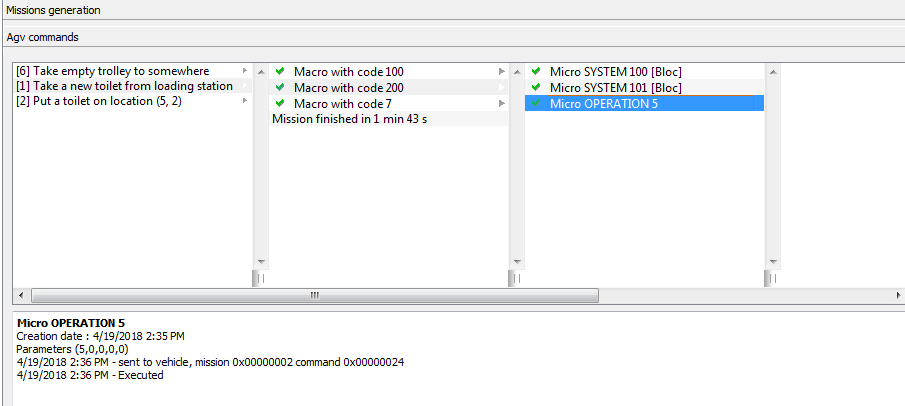
\includegraphics[scale=0.5]{agvmanager/agvManager/microDebug}
	\caption{Macro expansion and micro details}
	\label{figmacroexp}
\end{figure}
%------------------
%
%------------------
\subsection{Micros and Operations}
Micros are low level set of instructions. The following listing.\ref{lstMIC} show the different categories of micro instructions or operations defined by AgvManager. 

\begin{lstlisting}[caption= Different catergory of MIC defined in AgvManager, label=lstMIC]
// Definizione codici micro
$define MIC_NULL              0
$define MIC_MOVE              1 // M command, agvregisterMove****
$define MIC_CURVE             2 // M command
$define MIC_ROTATION          4 // M command
$define MIC_OPERATION         5 // O command, agvregisterOperation()
$define MIC_SYSTEM            6 //   command are not sent to vehicle, agvregistersystembloccante(), agvregistersystempassante()
$define MIC_PASSANTE          7 // P command, agvregisterPassante()
$define MIC_WAIT              8 // W command, agvregisterWait()
$define MIC_MOVING_OPERATION  9 // Q command, agvregisterMovingOperation()

\end{lstlisting}

The following are MICROs defined by AgvManger.

\begin{lstlisting}[caption= MICRO and OPERAIONS defined by AgvManager]
// Definizione codici operazioni
$define O_LOAD          2
$define O_UNLOAD        3
$define O_CHARGE        4
$define O_CHARGE_START  1
$define O_CHARGE_STOP   2

// Definizione codici micro System
$define S_NULL          0	// Serve (ad esempio) a spezzare le MIC_MOVE
$define S_END           1
$define S_CHARGE_WAIT   3
$define S_CHARGE_START  4
$define S_CHARGE_STOP   5
$define S_CONCAT_MACRO  8	// Concatena immediatamente la macro successiva
\end{lstlisting}

We can define are own Micros and operations. Try to follow the naming style of AgvManager. Begin with the prefix O\_ for Operation category, with S\_ for System category.

\begin{lstlisting}[caption= MICRO and OPERAIONS defined by user]
//	Micro SYSTEM
$define S_START_WAIT		100
$define S_EXEC_WAIT			101

//	Micro OPERATION
// Wait toilet on agv
$define O_WAIT_TOILET		5
\end{lstlisting}

Micros form category MIC\_OPERATION, MIC\_SYSTEM, MIC\_PASSANTE, MIC\_WAIT are assigned in onExpandMacro(), using one of the following functions:
\begin{lstlisting}
	AgvRegisterPassante()
	AgvRegisterWait()
	AgvRegisterSystemPassante()
	AgvRegisterSystemBloccante()
\end{lstlisting}

Micros that belong to MIC\_MOVE, MIC\_CURVE, MIC\_ROTATION are assigned by AgvMoveTo****() functions.

Micro execution is done in onExecuteMicro(), for example:

\begin{lstlisting}
case MIC_SYSTEM
	case S_END
		; End of mission
		AgvStopMission(uAgv)
		SetAgvMessage(uAgv, "")
		break
		
	case S_START_WAIT
	// start timer. Not locking micro
		timerWait[uAgv] = timeoutS(iPar1)
		break
	
	case S_EXEC_WAIT
	// wait a timer to finish counting. locking micro
		if (isTimeout(timerWait[uAgv]))
			return true
		else
			MultiMessageState(uAgv, "Agv " + (uAgv + 1) + " : wait " + int(secsToTimeout(timerWait[uAgv])) + "s")
		return false
		endif
		break
	
	case S_WAIT_INPUT
	// wait a signal from plc. locking micro
		if ( AgvGetInput(INP_LOAD_TERMITAED) =false )
			return true
		else
			return false
		endif

\end{lstlisting}

Keep in mind that when a micro terminate, onExecuteMicro() should return true. For example, if we are waiting for a signal to be false, and the signal is true, onExecuteMicro() return false, in this way the next micro will be the current one.
When the signal become false, onExecuteMicro() return true and the execution of the current micro terminate.

When bLastCall will be set to true? at the next execution or immediately, and the effective termination will be at the next call?

For example if we register a micro from the category Operation, AgvManager will send some command to the vehicle. When the vehicle answer with operation concluded, AgvManager will set bLastCall to true, in this way we can terminate the micro execution.

From AgvManager we can send command to agv from the interpreter box. For example the operation command structure is: [Occccmmmm,type,p1,p2,p3,p4]. For example [O\textcolor{blue}{0001}\textcolor{red}{0003},1,0,0,0,0], fig.\ref{fig:operationCmd}, we send to Agv an operation command [O], with operation number 1 and mission number 3.

\begin{figure}
	\centering
\includegraphics[scale=0.4]{agvmanager/agvManager/operationCmd}
	\caption{Commands insertion}
	\label{fig:operationCmd}
\end{figure}

Details about mission, macro and micro execution can be seen in the tab vehicle informations[F3]. 

%------------------
%
%------------------
\subsection{Store handling}
In a matrix store, or stack, products can be taken out following the logic of First in First out (FIFO) or Last in First out(LIFO), etc.

We can define some objects to handle the store, keep in memory the products in the store and track them, and also some algorithm to take out or take in products.


%----------------------------------------------------------------------------------------
%
%----------------------------------------------------------------------------------------














